\documentclass{article}
\usepackage{xepersian}
\usepackage{listings}
\usepackage{xcolor}
\usepackage{graphicx}
\usepackage{caption}
\usepackage[margin=3.6cm]{geometry}

\lstset{
    tabsize = 4,
    showstringspaces = false,
    commentstyle = \color{green},
    keywordstyle = \color{blue},
    stringstyle = \color{red},
    rulecolor = \color{black},
    basicstyle = \small \ttfamily,
    breaklines = true,
}

\settextfont{XB Yas}

\title{\textbf{گزارش‌کار پروژۀ عید - برنامه‌سازی پیشرفته (جاوا)}\vspace{1cm}\\پاسخ سوالات قدم دوم}
\author{\textbf{پیشوا آزیز - \lr{40313003}}}
\date{}

\begin{document}

\maketitle

\vspace{2cm}

\section*{پاسخ سوال ۱}

Shallow copy و Deep copy به مفاهیم مربوط به کپی کردن آبجکت‌ها برمی‌گردد. وقتی سعی می‌کنیم آبجکتی را کپی کنیم و آن‌را در جایی دیگر ذخیره کنیم باید در مورد این موضوع یعنی نوع کپی کردن آگاهی داشته باشیم.
Shallow copy را با یک مثال بهتر متوجه می‌شویم:

فرض کنید کلاسی با نام \lr{\lstinline{Person}} داریم که در آن یک فیلد از نوع \lr{\lstinline{Address}} که آن هم خود یک کلاس است، وجود دارد.

\begin{latin}
\begin{lstlisting}[language = Java, firstnumber = last, escapeinside={(*@}{@*)}]
class Address {
    public String city;
    public String country;

    public Address(String city, String country) {
        this.city = city;
        this.country = country;
    }
}

class Person {
    public String name;
    public Address address;

    public Person(String name, Address address) {
        this.name = name;
        this.address = address;
    }

    public Person copy() {
        return new Person(this.name, this.address);
    }
}
\end{lstlisting}
\end{latin}

شاید این‌گونه به نظر برسد که متد \lr{\lstinline{copy}} می‌تواند آبجکتی جدید از نوع \lr{\lstinline{Person}} بازگرداند و مشکلی در پیاده‌سازی آن وجود ندارد. در حالی که با تست کردن عملکرد آن می‌توان متوجه شد که مشکل آن چیست. حال با ساختن یک آبجکت از نوع \lr{\lstinline{Person}} و کپی کردن آن در آبجکتی دیگر با استفاده از متد \lr{\lstinline{copy}} کدی مانند زیر خواهیم داشت:

\begin{latin}
\begin{lstlisting}[language = Java, firstnumber = last, escapeinside={(*@}{@*)}]
public class Main {
    Address location = new Address("Hewler", "Kurdistan");
    Person person1 = new Person("Hozan", location);
    Person person2 = person1.copy();

    person2.name = "Dilan";
    person2.address.city = "Amed";

    System.out.println(person1.name + " is from " + person1.address.city);
    System.out.println(person2.name + " is from " + person2.address.city);
}
\end{lstlisting}
\end{latin}

با مشاهدۀ خروجی این کد، می‌توان فهمید تغییری که در یکی از فیلدهای \lr{\lstinline{person2}} انجام شد، باعث همین تغییر در \lr{\lstinline{person1}} نیز شده است. البته این فیلد از نوع \lr{\lstinline{Address}} بوده و به دلیل این که رفرنس آن از \lr{\lstinline{person1}} به \lr{\lstinline{person2}} کپی شده است، تغییرات یکسانی داشته‌اند؛ وگرنه تغییری که در \lr{\lstinline{person2.name}} اعمال شده است، موجب تغییر در \lr{\lstinline{person1.name}} نشده است، چون فیلد \lr{name} از نوع \lr{primitive} است. لذا آبجکت‌ها و رفرنس‌های داخلی هر آبجکت همان‌گونه باقی مانده‌اند و نسخه‌های جدیدی از آن‌ها به‌وجود نیامده است. این نوع کپی کردن که در آن آبجکت کپی‌شده، با همان رفرنس‌های داخلی قبلی کپی می‌شود، \lr{Shallow copy} می‌باشد.

این موضوع در این‌جا، با توجه به مشکلی که در پایان قدم اول پروژه مشاهده شد، در اصل نوعی عملکرد نامطلوب دیتابیس است، لازم است تا متد مربوط به کپی کردن آبجکت‌ها به گونه‌ای صحیح پیاده‌سازی شود تا رفرنس‌هایی که در آبجکت‌ها مورد استفاده قرار گرفته است، متمایز از هم باشند و به یک فضای واحد در حافظه اشاره نکنند.

با این توصیف، می‌توان پیش‌بینی کرد که \lr{Deep copy} چه تمایزاتی دارد. \lr{Deep copy} به نوعی از کپی کردن آبجکت‌ها اشاره می‌کند که در آن، از رفرنس‌ها و آبجکت‌های داخلی هم کپی گرفته می‌شود و به‌جای هر کدام از آن‌ها، نسخه‌های جدیدی در آبجکت کپی‌شده قرار می‌گیرند. برای این منظور می‌توان پیاده‌سازی متد \lr{\lstinline{copy}} را به شیوۀ زیر تغییر داد:

\begin{latin}
\begin{lstlisting}[language = Java, firstnumber = last, escapeinside={(*@}{@*)}]
public Person copy() {
    Person copied = (Person) super.clone();
    copied.address = new Address(this.address.city, this.address.country);
    return copied;
}
\end{lstlisting}
\end{latin}

همان‌گونه که مشاهده می‌شود، نسخۀ جدیدی از فیلد \lr{\lstinline{address}} که از نوع \lr{reference} می‌باشد، ایجاد شده است. با این نوع پیاده‌سازی، دیگر هرگونه تغییر در هر یک از فیلدهای آبجکت‌های \lr{\lstinline{person1}} یا \lr{\lstinline{person2}}، تاثیری بر دیگری نمی‌گذارد.

\section*{پاسخ سوال ۲}

در اینجا به‌خاطر یکی از قابلیت‌های جاوا به نام \lr{Covariant return types}، می‌توان نوع خروجی از متد‌ها را تغییر داد، به شرطی که موارد زیر برقرار باشند:

\begin{enumerate}
    \item نوع خروجی از متد \lr{override}کننده، باید یک زیرکلاس از نوع خروجی متد \lr{override}شده باشد.
    \item این تغییر سیگنچر فقط برای \lr{reference type}ها پاسخ‌گو است و برای \lr{primitive type}ها امکان‌پذیر نمی‌باشد.
\end{enumerate}

با توجه به موارد بالا، چون کلاس \lr{\lstinline{Human}} زیرکلاسی از کلاس \lr{\lstinline{Entity}} است، می‌توان نوع خروجی متد \lr{\lstinline{copy}} را از \lr{\lstinline{Entity}} به \lr{\lstinline{Human}} تغییر داد.

\section*{پاسخ سوال ۳}

\begin{figure}[h]
\begin{latin}
\centering
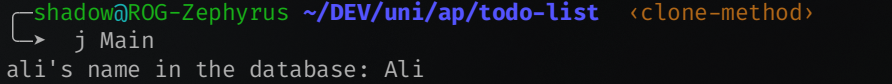
\includegraphics[width=0.7\textwidth]{../img/screenshot1.png}
\end{latin}
\caption*{اسکرین‌شات از خروجی کد حین اجرای بخش تست کد}
\end{figure}

\section*{پاسخ سوال ۴}

متد \lr{\lstinline{clone}} در جاوا برای ایجاد کپی از یک آبجکت استفاده می‌شود. این متد در کلاس \lr{\lstinline{Object}} تعریف شده است. برای استفاده از آن شرایطی مانند \lr{implement} کردن اینترفیس \lr{\lstinline{Cloneable}} توسط کلاس مورد نظر (برای جلوگیری از اکسپشن مربوطه) و \lr{override} کردن متد \lr{\lstinline{clone}} و فراخوانی \lr{\lstinline{super.clone()}} وجود دارد. استفاده از این متد به تنهایی، آبجکت مورد نظر را صرفا \lr{Shallow copy} می‌کند و برای پیاده‌سازی \lr{Deep copy} باید به صورت دستی رفرنس‌های موجود در داخل آبجکت‌ها را کپی کرد.

\section*{پاسخ سوال ۵}

مطابق سورس‌کد خود جاوا، اینترفیس \lr{\lstinline{Cloneable}} هیچ متدی در تعریف خود ندارد و استفاده از آن برای کلاسی که متد \lr{\lstinline{clone}} را پیاده‌سازی می‌کند صرفاً جنبۀ مارکر دارد و نشان می‌دهد که کلاس ذکرشده از \lr{cloning} پشتیبانی می‌کند.

از طرفی ضرورت استفاده از این اینترفیس می‌تواند به مفاهیم \lr{clean code} به‌خصوص واضح‌تر شدن و جلوگیری از عملکرد غیرمنتظره و نامطلوب مربوط شود.

\end{document}